\section{phase$\_$6}

	\begin{itemize}
	
	\item
	
	第六关的汇编代码如下:
		
	\lstinputlisting[language={[x86masm]Assembler}]{sources/phase_6.asm}

	\item
	
	首先发现它调用了\textbf{strtol}这个函数。观察这个函数的代码发现,它需要传入三个参数,这里分别为\textbf{$\%eax$, 0 和 0xa}。\textbf{strtol}的主要功能可以用以下c语言代码表示:

	\lstinputlisting{sources/strtol.txt}	
	
	这段代码的作用就是将输入的字符串转换为对应的base进制数表示。

	\item
	
	\lstinputlisting[language={[x86masm]Assembler}]{sources/phase_6_part_1.asm}
	
	这里调用了函数\textbf{fun6}。由于传入的是一个地址\textbf{0x804c174},因此fun6的返回值是固定的,因此,经过一系列跳转后,在\textbf{cmp $\%$edx, ($\%$eax)}中, ($\%$eax)的值也是一定的。运用gdb设置断点,查看得知此时($\%$eax)的值为268。

	\item	

	由于$\%$edx的值就是我们输入的字符串,答案就唾手可得了。
	
	\end{itemize}
	
	输入\textbf{268},顺利过关。
	
	\begin{figure}[h]
		\centering
			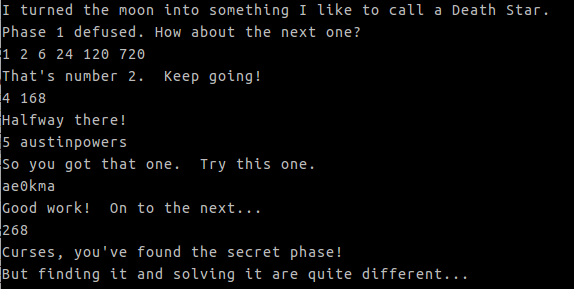
\includegraphics[scale=0.77]{images/phase_6_success.png}
	\end{figure}	
